% !TeX root = root.tex
% !TeX spellcheck = en_US
\section{Permutation groups as automorphism groups of graphs}

\subsection*{a)}
$\Omega = \{1,2,3,4,5,6\}$, $<(1,2,3)(4,5,6)>$, this is simple to argue, with this generator you cant interchange elements from the two cycles and the only way of making one of the cycle is with a directed cycle in a graph, however if you make two directed cycles they are interchangable.

\subsection*{b)}
The Cayley graph from the lecture has this propperty if the edges are colored. We then simply have to reform the graph with methods from algorithms and symmetry to remove the color but have equivalent automorphisms.

\subsection*{c)}
For this task we consider a graph with 3 sets of vertices from $\Omega$. Firstly we have all elements from $\Omega$ labeled with their number, we will call these base, secondly we have all elements from $\Omega$ without labels, we will call these map, lastly we have all elements from $\Omega$ without labels again, we will call these equivalence. The idea is to connect the base with the map to simulate a permutation. We will have multiple maps for each permutation in the group one. Now to connect all of the maps somehow we use the equivalence. Each vertex in each map is connected to itself from the equivalence. This will allow us to represent each permutation with an automorphism on the equivalence (An example can be seen in Figure \ref{fig:1} ).

To argue the correctness we simply observe, because of the labels base has to be mapped to base. Now after we map the equivalence all of the map are fixed and thus any automorphism is isomorphic to an element in $Sym(\Omega)$. Now for any automorphism $\phi \simeq h\in Sym(\Omega)$, the map have to be mapped to each other and if they can be mapped to each other this is equivalent to saying $\forall g \in G: gh \in G$, and this is only true for $h \in G$.

\begin{figure}
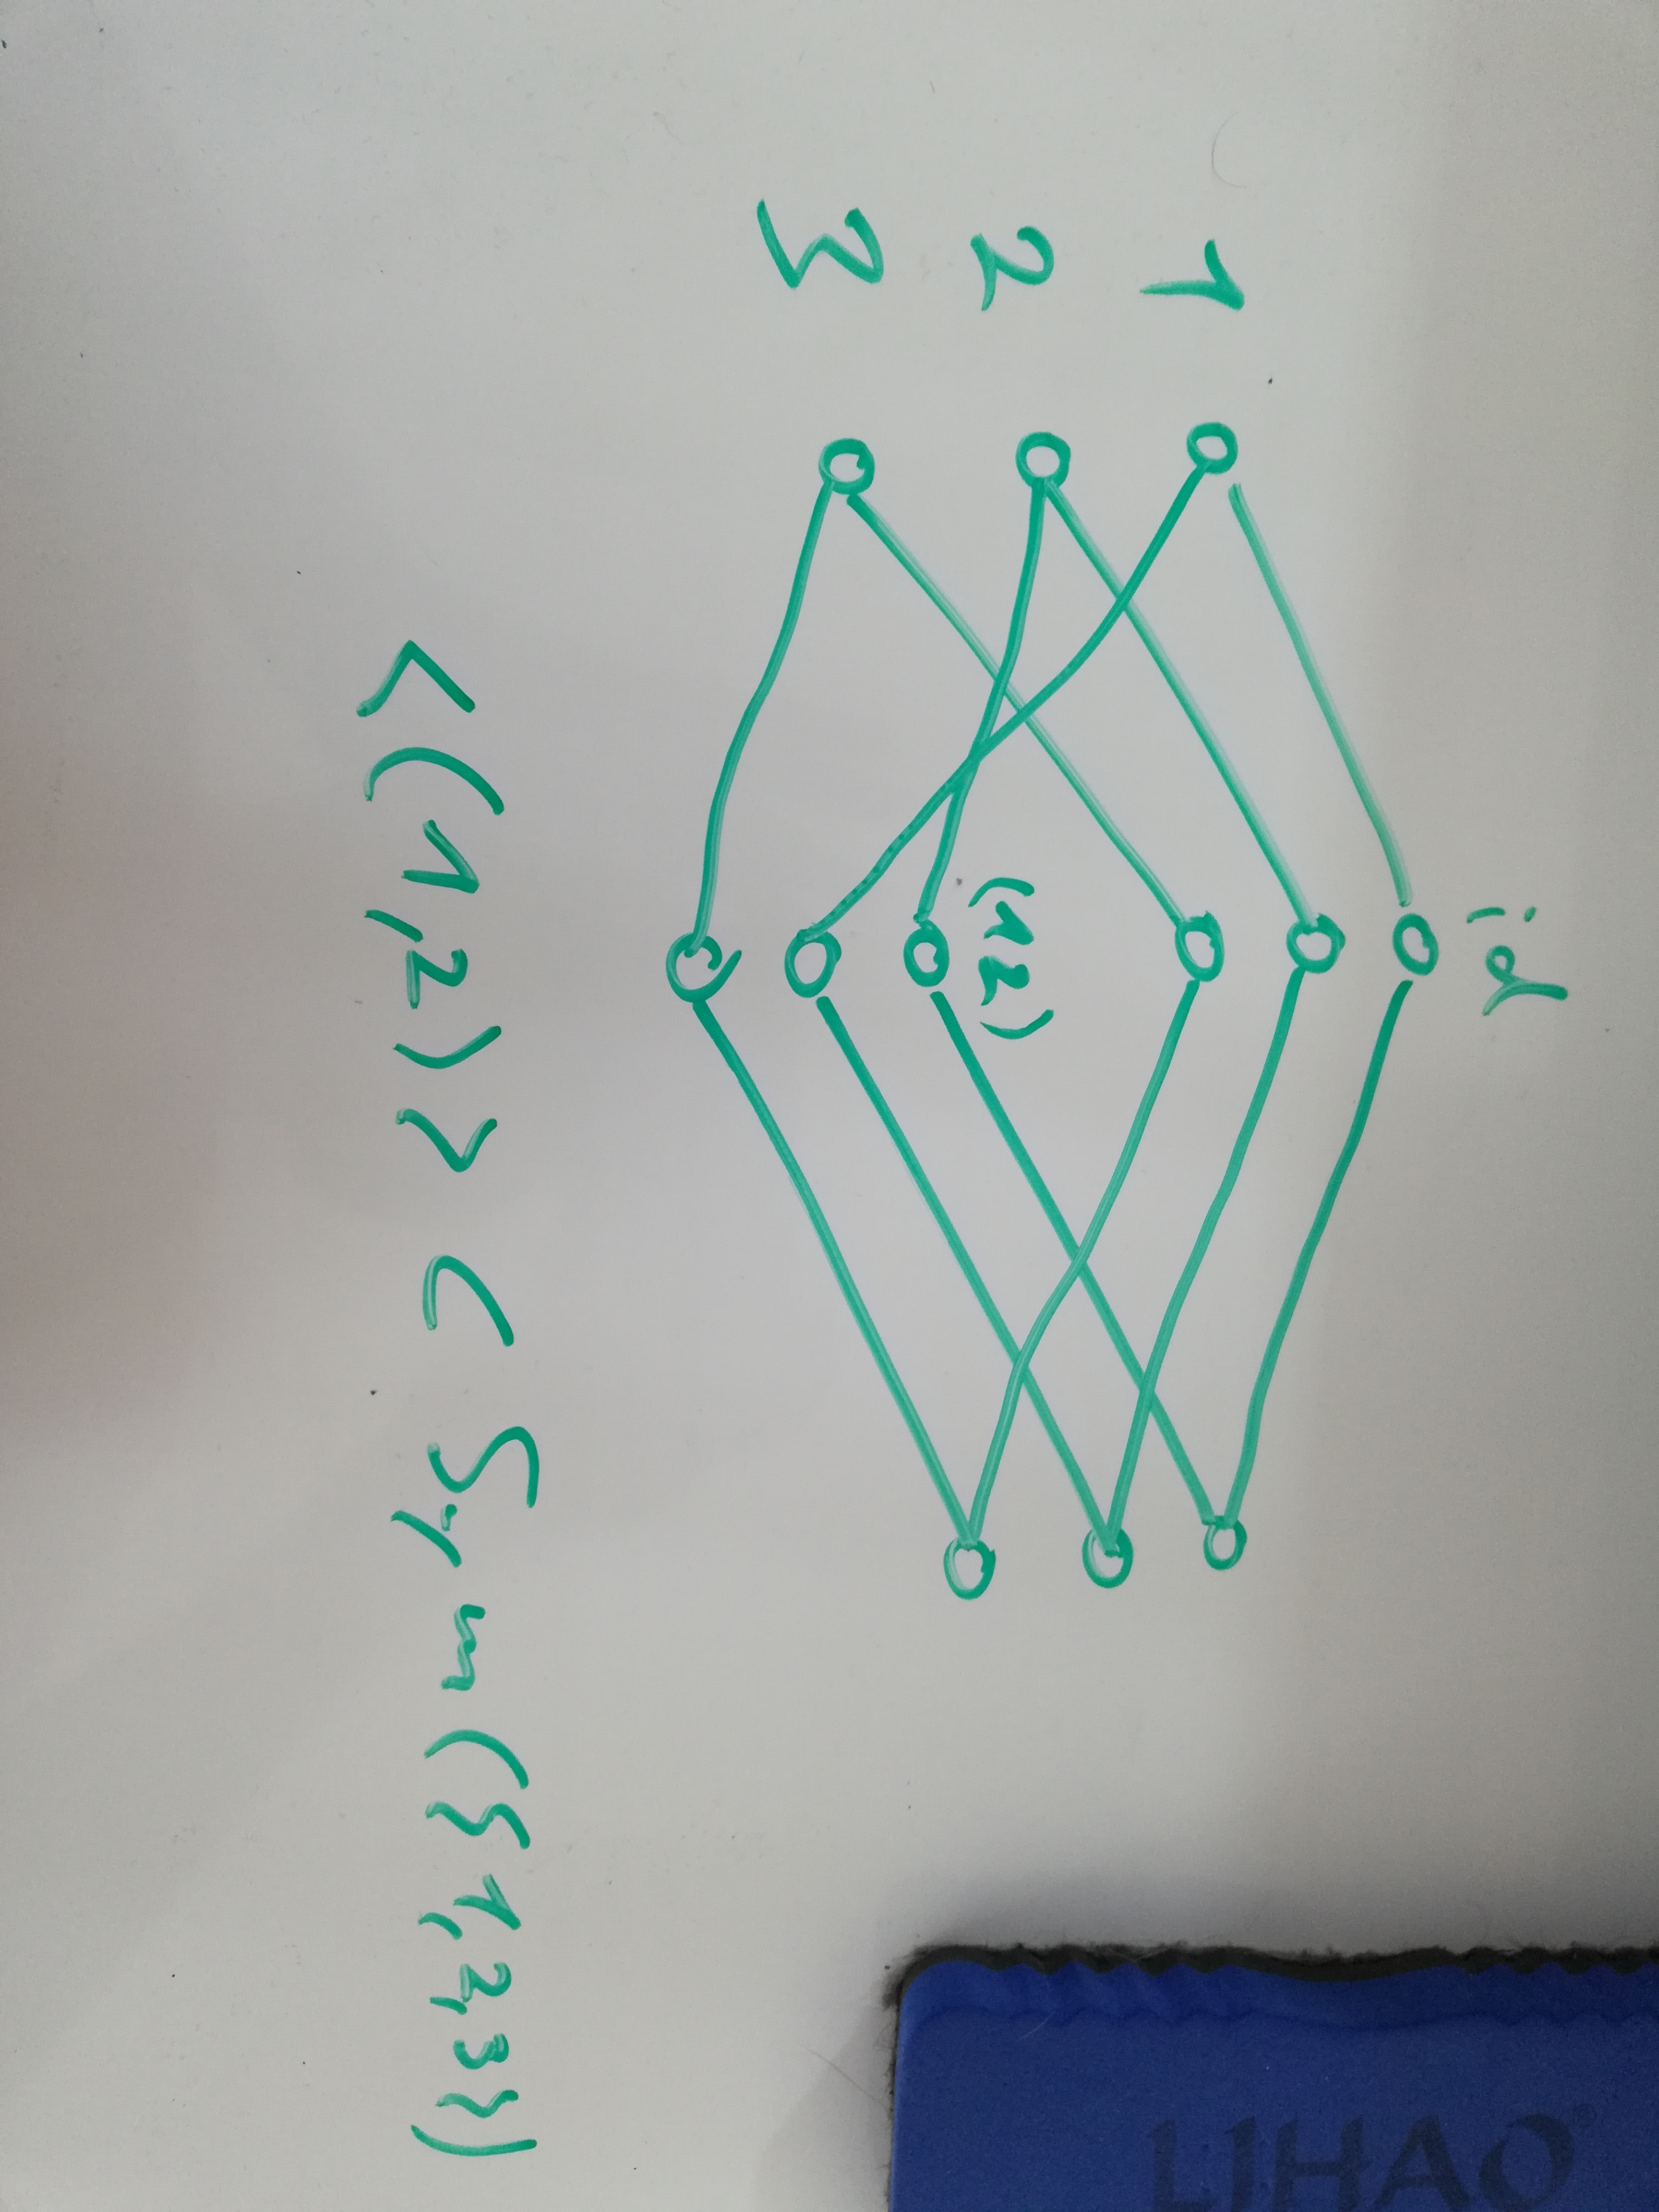
\includegraphics[height=\textwidth, angle=90]{graph.jpg}
\caption{Picture for exercise 1}
\label{fig:1}
\end{figure}